% =============================================================================
% Lecture 11b: Hardware Acceleration, Part 2 (Mapping a Computation onto the Chip)
% Introduction to Machine Learning Systems (Volume I)
% =============================================================================
% A chip reaches the ceiling its roofline promises only when the mapping keeps
% the right operand in the right tier: the loop order picks what stays, the
% tile sets reuse within on-chip capacity, shapes must fill whole tiles and
% whole waves, and a compiler searches these choices for every layer.
%
% Build: make -C slides build-11b_hw_acceleration   (figures: images/make_figs.py)
% Plan:  lecture_map.yml and storyboard.md in this folder.
% =============================================================================

\documentclass[aspectratio=169, 12pt]{beamer}
\usepackage{../../assets/beamerthememlsys}
\mlsyssetup{
  volume={Volume I},
  chapter={Chapter 11},
  chaptertitle={Hardware Acceleration, Part 2},
  logo={../../assets/img/logo-mlsysbook.png},
  instlogo={../../assets/img/logo-harvard.png},
  layer=hardware,
}
\usepackage[T1]{fontenc}
\usepackage[scaled=0.9]{helvet}
\usepackage{courier}
\renewcommand{\familydefault}{\sfdefault}
\usepackage{booktabs,amsmath}
\graphicspath{{images/}}
\setcounter{mlsystotalsections}{4}

\title{Hardware Acceleration, Part 2}
\author{Vijay Janapa Reddi}
\institute{Harvard University}
\date{}

% A large answer choice for predict and concept-question slides
\newcommand{\choice}[2]{\textbf{\textcolor{mlsysaccent}{#1}}\enspace #2}
% A goal or takeaway line with its thumbnail
\newcommand{\thumbline}[2]{%
  \begin{minipage}[c]{2.6cm}\centering\includegraphics[width=2.5cm,height=1.05cm,keepaspectratio]{#1}\end{minipage}%
  \hspace{0.3cm}\begin{minipage}[c]{0.74\textwidth}\normalsize #2\end{minipage}}
% A true-or-false statement card
\newcommand{\tfcard}[2]{%
  {\small\textbf{#1}}\\[0.05cm]
  \uncover<2->{\footnotesize\textcolor{RedLine}{\textbf{False.}} #2}\\[0.3cm]}
% One line of code in a loop-order column
\newcommand{\cl}[1]{{\ttfamily #1}\\}
% A row of the per-order traffic table, shown from overlay #1 on
\newcommand{\trow}[5]{\uncover<#1->{#2} & \uncover<#1->{#3} & \uncover<#1->{#4} & \uncover<#1->{#5} \\}
% The saved operand in a traffic row
\newcommand{\saved}[1]{\textcolor{GreenLine}{\textbf{#1}}}
% A tier row in the activation-trip table: tier, what it holds, what decides
\newcommand{\tier}[3]{\textbf{#1} & #2 & #3 \\}

\begin{document}

% =============================================================================
% TITLE AND HOOK
% =============================================================================
\mlsysnote{[0.5 min] Read the thesis aloud once. Part 1 built the machine and its two ceilings. Today asks how a computation reaches those ceilings: which operand stays next to the arithmetic, how large a block fits on chip, what happens when a shape does not divide evenly, and who makes these choices for every layer. The notes total about 70.5 minutes, which leaves a few minutes for questions. FLEX: the [OPTIONAL] frames give a 60-minute version.}
\mlsystitle{Hardware Acceleration, Part 2}{A chip reaches its roofline only when the mapping keeps the right operand in the right tier.}{cover_hw_acceleration_blueprint.png}

\begin{frame}{How much faster can one GPU run the same multiply?}
  \mlsysactivity{Predict}{2 min}
  \centering
  \mlsyssteps[width=0.95\textwidth,height=3.2cm,keepaspectratio]{hook_step}{2}\\[0.15cm]
  \raggedright\small One FP32 matrix multiply, about 4,096 square, on one RTX A6000. A naive CUDA kernel reaches 309 GFLOP/s. How fast does NVIDIA's cuBLAS library run it?\\[0.15cm]
  \centering\normalsize\choice{A}{2$\times$}\qquad\choice{B}{10$\times$}\qquad\choice{C}{75$\times$}\qquad\choice{D}{1,000$\times$}\\[0.15cm]
  \uncover<2->{\normalsize Same chip, same arithmetic, same answer.}
  \mlsyscredit{Boehm, ``How to Optimize a CUDA Matmul Kernel for cuBLAS-like Performance: a Worklog,'' 2022 (siboehm.com), results table; GPU and matrix size from the article's text. 75$\times$ derived.}
  \note{[3.5 min] Step 1: a naive kernel gives each GPU thread one output element; it reaches 309 billion floating-point operations per second (GFLOP/s). ENGAGE: vote with fingers before the reveal. Step 2: C. cuBLAS reaches 23,250 GFLOP/s, 75 times faster, on the same GPU with the same arithmetic and the same result. Simon Boehm wrote eight faster kernels between the two, and none of them does less arithmetic. Each changes where operands live and how often they cross a memory boundary: coalesced loads (neighboring threads read neighboring addresses) gave 6.4 times, tiles staged in shared memory 1.5, larger register tiles 2.8 and then 1.9, and wider loads, autotuning, and tiles per warp (a group of 32 threads) the rest. WARN: D is the belief that the gap is hardware; A is the belief that a correct kernel is a fast one. These are FP32 results without Tensor Cores, from one engineer's worklog on one GPU. LINK: Part 1 gave the ceiling; today is the schedule that reaches it. The synthesis returns to this ladder. FLEX: [CORE].}
\end{frame}

\begin{frame}{Recall: what did the roofline promise the stage-3 conv?}
  \mlsysactivity{Recall}{1.5 min}
  \begin{columns}[c]
    \begin{column}{0.40\textwidth}
      {\Large\bfseries Close your notes.}\\[0.3cm]
      \small H100, FP16:\\[0.1cm]
      What is the ridge point?\\[0.1cm]
      Where does ResNet-50's stage-3 3$\times$3 conv sit at batch 32?\\[0.1cm]
      What rate does the roofline allow it?
    \end{column}
    \begin{column}{0.58\textwidth}
      \centering
      \uncover<2->{\safeimg[width=\textwidth,height=3.9cm,keepaspectratio]{recall_roof.pdf}\\[0.1cm]
        {\small Ridge 295; conv 563 FLOP/byte; ceiling 989 TFLOP/s.}}
    \end{column}
  \end{columns}
  \mlsyscredit{Hardware Acceleration, Napkin Math 11.5 and 11.10.}
  \note{[1.5 min] ENGAGE: 45 seconds, written, notes closed. Step 2: the H100's FP16 ridge is 295.2 FLOP/byte (989 TFLOP/s over 3.35 TB/s). The stage-3 convolution does 563.1 FLOP per byte at batch 32, above the ridge, so the roofline allows it up to the 989 TFLOP/s FP16 ceiling. Say the open part: the roofline assumes the best schedule. It does not say what that schedule is, or who finds it. That is today. LINK: Lecture 11, Part 1. FLEX: [CORE].}
\end{frame}

\begin{frame}{How does a computation get mapped onto the chip?}
  \vspace{-0.1cm}
  {\normalsize By the end of today you will be able to:}\\[0.25cm]
  \thumbline{trace2_step5}{Trace a systolic array cycle by cycle and estimate how much input keeps it busy.}\\[0.15cm]
  \thumbline{capacity_step4}{Count the traffic of a loop order and a tile, and test a tile against on-chip capacity.}\\[0.15cm]
  \thumbline{wave_step2}{Predict what a shape one past a tile, or one past a wave, costs.}\\[0.15cm]
  \thumbline{compiler_step4}{Say what a compiler decides, and diagnose a kernel that misses its fast path.}
  \note{[1.5 min] The driving question: how does a computation get mapped onto an accelerator's arrays and memory tiers, and what does each choice cost? Read the four outcomes; each thumbnail is the figure that teaches it. Three running cases at three scales: the multiply from the hook; the chapter's dense layer (512 by 256 weights, a batch of 32), which carries the traffic counts; and ResNet-50 on the H100, which carries the compiler and the closing trip of one activation map. FLEX: [CORE].}
\end{frame}

% =============================================================================
% SECTION: THE ARRAY
% =============================================================================
\mlsysnote{[0.5 min] Start inside the array that Part 1 drew as a static picture. Read the divider question. The stack on the left shows where today sits: the hardware layer, as in Part 1.}
\mlsysdivider{What happens inside a systolic array, cycle by cycle?}{Hardware Acceleration, \S11.4.4, \S11.7.4, \S11.7.5 (the 2$\times$2 trace)}
\section{The Array}

\begin{frame}{Skewed inputs make the right operands meet}
  \mlsysactivity{Predict}{1 min}
  \centering
  \mlsyssteps[width=\textwidth,height=5.15cm,keepaspectratio]{trace2_step}{5}\\[0.05cm]
  \small
  \only<1|handout:0>{$C = AB$ on a 2$\times$2 array: PE$_{rc}$ holds weight $b_{rc}$.}%
  \only<2|handout:0>{In cycle 1, $a_{00}b_{00}$ moves down to PE$_{10}$, which holds $b_{10}$. Which activation must meet it?}%
  \only<3|handout:0>{$a_{01}$: it enters row 1 one cycle after $a_{00}$ entered row 0.}%
  \only<4|handout:0>{$C_{01}$ leaves one cycle after $C_{00}$; the second input row follows one cycle behind.}%
  \only<5-|handout:1>{Each row starts one cycle later, so operands with the same reduction index meet.}
  \mlsyscredit{Hardware Acceleration, \S11.7.5 (the 2$\times$2 trace) and figure 5; Kung 1982. $C_{10}$ and $C_{11}$ follow the same stagger.}
  \note{[4.5 min] Step 1: Part 1's picture at 2 by 2. Each processing element (PE) holds one weight; activations move right, partial sums move down, one hop per cycle. $C_{00} = a_{00}b_{00} + a_{01}b_{10}$. Step 2, cycle 0: $a_{00}$ meets $b_{00}$ in PE00. ENGAGE: in cycle 1 that product moves down to PE10, which holds $b_{10}$. Which activation must be there, and when must it enter? Step 3: $a_{01}$, entering row 1 one cycle late. PE10 adds its product and $C_{00}$ leaves. Meanwhile $a_{00}$ moved right to PE01 and $a_{10}$ entered PE00. Step 4, cycle 2: $C_{01}$ and $C_{10}$ leave. Step 5, cycle 3: $C_{11}$ leaves. Two input rows took four cycles on a 2 by 2 array. WARN: students picture every cell starting at once; the skew is what makes the right operands meet. FLEX: [CORE].}
\end{frame}

\begin{frame}{A 4$\times$4 array fills, runs full, then drains}
  \centering
  \mlsyssteps[width=\textwidth,height=5.7cm,keepaspectratio]{wave4_step}{3}
  \mlsyscredit{Derived from Hardware Acceleration, \S11.7.5 (one hop per cycle). Weight loading not shown.}
  \note{[2.5 min] The same timing on a 4 by 4 array streaming 8 input rows through one set of weights. Each cell shows which input row it is working on. Step 1, cycle 2: only the top-left corner has work; 6 of 16 cells are busy. Step 2, cycle 6: the wavefront covers the array; all 16 cells are busy, but only for cycles 6 and 7. Step 3, cycle 11: the array drains from the top left; 6 cells are busy again. Eight rows take 8 + 2(4) $-$ 2 = 14 cycles, so the cells are busy 57 percent of the time on average. ENGAGE: what would raise that share? Expected: more input rows per weight load. WARN: the count ignores the cycles to load the weights themselves, which makes the real share lower. FLEX: [OPTIONAL]; if cut, state the B + 2N $-$ 2 count on the next frame.}
\end{frame}

\begin{frame}{A 128$\times$128 array needs hundreds of rows per load}
  \mlsysactivity{Estimate}{1.5 min}
  \begin{columns}[c]
    \begin{column}{0.37\textwidth}
      \begin{mlsyscard}{mlsysaccent}
        \textbf{Given}\\[0.1cm]
        $N\times N$ array, $B$ input rows\\
        Cycles: about $B + 2N - 2$\\
        Busy: $B \,/\, (B + 2N - 2)$\\
        $N = 128$
      \end{mlsyscard}
      {\footnotesize Busy fraction at $B$ = 1, 128, 1,024?}
    \end{column}
    \begin{column}{0.61\textwidth}
      \centering
      \uncover<2->{\safeimg[width=\textwidth,height=3.6cm,keepaspectratio]{busy.pdf}\\[0.1cm]
        {\small One row uses 0.4\% of the array.}}
    \end{column}
  \end{columns}
  \mlsyscredit{Derived from Hardware Acceleration, \S11.7.5; 128$\times$128 as in TPU v4 (Jouppi et al. 2023). Idealized: weight loading ignored.}
  \note{[2.5 min] ENGAGE: one minute in pairs. The count generalizes the last slide: B rows take B cycles to enter, plus about 2N $-$ 2 cycles to fill and drain. Step 2: for a 128 by 128 array, the size in a TPU v4 core, one row keeps it busy 0.4 percent of the time, 128 rows 34 percent, 1,024 rows 80 percent, and 4,096 rows 94 percent. These are derived, and idealized, since loading each weight tile costs about N more cycles. This is why a weight-stationary array wants a large batch, or many output positions per weight as in a convolution. WARN: the batch that fills the array also makes requests wait for each other. LINK: Lecture 13 owns that trade between throughput and latency. FLEX: [CORE].}
\end{frame}

\begin{frame}{The loop order decides which operand stays in the cell}
  \begin{columns}[T]
    \begin{column}{0.32\textwidth}
      \centering{\small\textbf{Weight stationary}}\\[0.05cm]
      \safeimg[width=0.92\textwidth,height=3.6cm,keepaspectratio]{stationary_ws.pdf}\\[0.05cm]
      \raggedright\scriptsize
      \cl{for i, k:}
      \cl{\ \ w = W[i,k]\ \textcolor{midgray}{\# 32 uses}}
      \cl{\ \ for j: Z[i,j]+=w*X[k,j]}
    \end{column}
    \begin{column}{0.32\textwidth}
      \uncover<2->{\centering{\small\textbf{Output stationary}}\\[0.05cm]
      \safeimg[width=0.92\textwidth,height=3.6cm,keepaspectratio]{stationary_os.pdf}\\[0.05cm]
      \raggedright\scriptsize
      \cl{for i, j:}
      \cl{\ \ for k: acc+=W[i,k]*X[k,j]}
      \cl{\ \ Z[i,j] = acc\ \textcolor{midgray}{\# once}}}
    \end{column}
    \begin{column}{0.32\textwidth}
      \uncover<3->{\centering{\small\textbf{Input stationary}}\\[0.05cm]
      \safeimg[width=0.92\textwidth,height=3.6cm,keepaspectratio]{stationary_is.pdf}\\[0.05cm]
      \raggedright\scriptsize
      \cl{for k, j:}
      \cl{\ \ x = X[k,j]\ \textcolor{midgray}{\# 512 uses}}
      \cl{\ \ for i: Z[i,j]+=W[i,k]*x}}
    \end{column}
  \end{columns}
  \mlsyscredit{Hardware Acceleration, listing 15 (abridged; W = weights 512$\times$256, X = input 256$\times$32, Z = output) and \S11.7.4.}
  \note{[3 min] The chapter's dense layer, $Z = WX$, 4,194,304 multiply-accumulates (MACs), in three loop orders. All compute the same result. Whatever the inner loops touch repeatedly without changing stays in the cell; everything else streams. Step 1: weight stationary holds one weight and streams inputs and partial sums past it; each weight is fetched once and used 32 times, once per batch column. This is the TPU's dataflow and the trace we just ran; the next slide counts one cell on its own first, then a row of cells. Step 2: output stationary holds a running sum; each output is written once, but weights and inputs both stream in. Step 3: input stationary holds one input, used 512 times, once per output row. ENGAGE: which order would you pick for one weight matrix applied to a large batch? Expected: weight stationary. WARN: no order captures all three reuses at once, because a cell holds one value. The next slide counts what each order still moves. FLEX: [CORE].}
\end{frame}

\begin{frame}{Holding one value saves one operand; neighbors save more}
  \centering\small
  \footnotesize One cell, no neighbors: what it does not hold comes from the slower tier.\\[0.1cm]
  \renewcommand{\arraystretch}{1.12}
  \begin{tabular}{@{}lrrr@{}}
    \toprule
    \textbf{Order} & \textbf{Weight reads} & \textbf{Input reads} & \textbf{Partial sums or outputs} \\
    \midrule
    \trow{1}{Weight stationary}{\saved{131,072}}{4,194,304}{8,388,608}
    \trow{2}{Output stationary}{4,194,304}{4,194,304}{\saved{16,384}}
    \trow{3}{Input stationary}{4,194,304}{\saved{8,192}}{8,388,608}
    \midrule
    \trow{4}{Weight stationary, row of 128 cells}{\saved{131,072}}{\saved{32,768}}{8,388,608}
    \bottomrule
  \end{tabular}\\[0.1cm]
  \begin{columns}[c]
    \begin{column}{0.38\textwidth}
      \raggedright\small
      \uncover<4->{Passing each input along a row of 128 cells divides input reads by 128.}
    \end{column}
    \begin{column}{0.58\textwidth}
      \centering
      \uncover<5->{\safeimg[width=\textwidth,height=1.8cm,keepaspectratio]{weight_reads.pdf}\\
        {\scriptsize The same loop-order effect in a convolution: 16 filters, 3$\times$3, on 8$\times$8}}
    \end{column}
  \end{columns}
  \mlsyscredit{Derived from Hardware Acceleration, listing 14 ($W$ 512$\times$256, $X$ 256$\times$32) and \S11.7.4: element moves; a partial sum is one read and one write per MAC; 4,194,304 / 128 = 32,768. Example 11.4 (modeled).}
  \note{[3 min] One row per step. The first three rows isolate the loop order: one cell, no neighbors, holding one value. Step 1: weight stationary reads each of the 131,072 weights once, but an input for every MAC, 4.2 million, and reads and writes a partial sum for every MAC, 8.4 million. Step 2: output stationary writes each of the 16,384 outputs once and streams 4.2 million weights and 4.2 million inputs. Step 3: input stationary reads each of the 8,192 inputs once. Each order saves one operand (green); the other two pay per MAC. ENGAGE: which of the three moves the fewest? Expected: output stationary, 8.4 million against about 12.6 million. Step 4: the array we traced. In a row of 128 weight-stationary cells each input enters once and passes past 128 held weights, so input reads fall to 4,194,304 / 128 = 32,768 (derived). A full array also passes partial sums down its columns, removing most of that traffic too. Step 5: Example 11.4. Holding all 16 filters over 36 output positions takes 144 weight reads; spilled, each position reloads all 144: 5,184 reads, 36 times more (modeled). WARN: real kernels hold a tile, the next segment. FLEX: [OPTIONAL] steps 1 to 3; keep step 4.}
\end{frame}

\begin{frame}{Holding several operands helps only where reuse exists}
  \mlsysactivity{Vote}{1.5 min}
  \centering
  \safeimg[width=0.66\textwidth,height=2.9cm,keepaspectratio]{eyeriss.pdf}\\[0.2cm]
  \uncover<2->{\raggedright\small GPT-2 XL decode, batch one, weight-stationary array: which change recovers weight reuse?\\[0.05cm]
    \choice{A}{Output stationary}\quad\choice{B}{Input stationary}\quad\choice{C}{Row stationary}\quad\choice{D}{None of them}}\\[0.15cm]
  \uncover<3->{\centering\small\textbf{D.} Each weight is used once per token. No reuse is left to recover.}
  \mlsyscredit{Chen, Emer, Sze, ``Eyeriss,'' ISCA 2016 (abstract; same area and parallelism); Hardware Acceleration, Systems Perspective 11.1.}
  \note{[2 min] Step 1: Eyeriss holds rows of weights, inputs, and partial sums together, a row-stationary dataflow. On AlexNet it used 1.4 to 2.5 times less energy than the other dataflows on convolutional layers, and at least 1.3 times less on fully connected layers above batch 16. Holding several operands pays because a convolution reuses all three. Step 2: ENGAGE: vote, discuss with a neighbor for 30 seconds, vote again. Step 3: D. At batch one each weight meets one input per token, so the levers are batching, fewer bytes per weight, or more bandwidth. Land the segment: inputs enter skewed so the right operands meet; the array is full only between fill and drain; the loop order picks which operand stays, and neighbors share what streams. FLEX: [CORE].}
\end{frame}

% =============================================================================
% SECTION: THE TILE
% =============================================================================
\mlsysnote{[0.5 min] One held value saves one operand. A block of values held on chip can save all three. Read the divider question.}
\mlsysdivider{How large a block fits on chip, and what happens at its edge?}{Hardware Acceleration, \S11.7.5 (equation 6); NVIDIA, Matrix Multiplication Background guide, \S3}
\section{The Tile}

\begin{frame}{Four weight tiles cut the layer's traffic 47 times}
  \begin{columns}[T]
    \begin{column}{0.40\textwidth}
      \centering\safeimg[width=0.95\textwidth,height=3.25cm,keepaspectratio]{layertile_mats.pdf}\\[0.1cm]
      \raggedright\scriptsize
      \uncover<4->{%
      \cl{for t in 0..3:\ \ \textcolor{midgray}{\# 4 weight tiles}}
      \cl{\ \ Ws = load W[128t:128t+128, :]}
      \cl{\ \ Xs = load X}
      \cl{\ \ for i in tile, j, k:}
      \cl{\ \ \ \ acc[i,j] += Ws[i,k]*Xs[k,j]}
      \cl{\ \ write Z rows of tile t}
      \textcolor{midgray}{Ws and Xs sit in shared memory.}}
    \end{column}
    \begin{column}{0.58\textwidth}
      \centering
      \mlsyssteps[width=\textwidth,height=5.5cm,keepaspectratio]{layertile_cost_step}{3}
    \end{column}
  \end{columns}
  \mlsyscredit{Derived from Hardware Acceleration, listing 14, listing 17 (abridged), and Lighthouse 11.2 (228 KB shared memory per H100 SM). FP16 operands, FP32 outputs.}
  \note{[4 min] The same layer on one H100 streaming multiprocessor (SM) with 228 KB of shared memory. Step 1: all the weights at FP16 are 256 KB and do not fit, so cut $W$ into four tiles of 128 rows. Step 2: one weight tile is 64 KB, the whole input 16 KB, one 128 by 32 FP32 output tile 16 KB: 96 KB, which fits. Step 3: load a weight tile once, stream the input past it, write its outputs once. Each weight is read once (131,072), the input four times (32,768), each output written once (16,384): 180,224 element moves against 8,404,992 untiled, about 47 times fewer. ENGAGE: why is the input read four times? Expected: once per weight tile. Step 4: the loop that makes a tile (listing 17, abridged). Each pass copies one weight tile and the input into shared memory, runs every multiply-add on the copies, and writes one block of outputs. This is explicit staging: the program decides what stays, as a GPU kernel does. A cache stages implicitly through the loop bounds alone (listing 16), and it can evict the tile before its reuse is done. WARN: derived counts for one SM. LINK: FlashAttention (Lecture 8b) tiles attention the same way. FLEX: [CORE].}
\end{frame}

\begin{frame}{A tile's edge sets how often each loaded byte is reused}
  \begin{columns}[c]
    \begin{column}{0.60\textwidth}
      \centering\safeimg[width=\textwidth,height=5.0cm,keepaspectratio]{tileintensity.pdf}
    \end{column}
    \begin{column}{0.38\textwidth}
      \centering
      \uncover<2->{{\small FP16 tiles, $T_M \times T_N$:}\\[0.2cm]
        {\large $I = \dfrac{T_M\,T_N}{T_M + T_N}$}\\[0.15cm]
        {\small FLOP per byte loaded}}
    \end{column}
  \end{columns}
  \mlsyscredit{Derived from Hardware Acceleration, \S11.7.5 (4,096-square FP16 multiply on 128-wide tiles); NVIDIA, Matrix Multiplication Background guide, \S2.3.}
  \note{[2 min] The chapter's 4,096 by 4,096 FP16 multiply, cut into 1,024 output tiles of 128 by 128, each summing 32 tile products. With no reuse every multiply-add reads two 2-byte operands: 0.5 FLOP per byte. With 128 by 128 tiles, each tile product loads two tiles, 65,536 bytes, and does 2 times 128 cubed, 4.19 million operations: 64 FLOP per byte. A 256 by 128 tile gives 85. Loading each matrix exactly once would give 1,365. Step 2: the formula: intensity grows with the tile's edge. NVIDIA's guide lists cuBLAS tiles from 256 by 128, the most efficient, down to 64 by 64, the least. ENGAGE: why not use the largest tile always? Expected: it must fit on chip, the next slide. WARN: a larger tile also leaves fewer tiles to spread across the chip. FLEX: [OPTIONAL] step 2.}
\end{frame}

\begin{frame}{Every live buffer must fit in the local store}
  \mlsysactivity{Estimate}{2 min}
  \centering
  {\normalsize $2\,T_M T_K + 2\,T_K T_N + 4\,T_M T_N \;\le\;$ local bytes}\\[0.05cm]
  {\small FP16 operands A, B; FP32 accumulator; a 228 KB local store. Does a 128$\times$128$\times$128 tile fit single buffered? Double buffered? With $T_K = 256$?}\\[0.15cm]
  \mlsyssteps[width=0.92\textwidth,height=3.8cm,keepaspectratio]{capacity_step}{4}
  \mlsyscredit{Derived from Hardware Acceleration, equation 6 (\S11.7.5); 228 KB budget from Lighthouse 11.2. 1 KB = 1,024 bytes.}
  \note{[3 min] Equation 6 counts every buffer that is live at the same time. ENGAGE: two minutes with a neighbor before step 2. Step 2: single buffered, A and B tiles are 32 KB each at FP16 and the FP32 accumulator 64 KB: 128 KB (131,072 bytes), fits. Step 3: double buffering loads the next pair of operand tiles while the current pair computes, so both operand buffers double: 192 KB, still fits. Step 4: doubling the reduction tile $T_K$ to 256 doubles both operand buffers again: 320 KB double buffered, over the budget, even though a longer reduction would amortize the accumulator. WARN: equation 6 imagines one local store. A GPU keeps accumulators in registers and budgets them separately, so the real shared-memory test counts only the operand copies (\S11.7.5). FLEX: [CORE].}
\end{frame}

\begin{frame}{A shape one past the tile pays for a whole tile}
  \mlsysactivity{Predict}{1 min}
  \begin{columns}[c]
    \begin{column}{0.40\textwidth}
      \centering\safeimg[width=\textwidth,height=4.2cm,keepaspectratio]{tiling.pdf}\\[0.05cm]
      {\footnotesize 1,024 tiles; 32,768 tile products}
    \end{column}
    \begin{column}{0.58\textwidth}
      \centering
      \only<1|handout:0>{\vspace{1.4cm}{\small A 4,096-wide layer on a 128$\times$128 array.}}%
      \only<2|handout:0>{\vspace{1.0cm}{\normalsize The layer width becomes \textbf{129}.\\[0.2cm] Array use along that dimension?}\\[0.3cm]{\Large\textbf{\textcolor{RedLine}{???}}}}%
      \only<3-|handout:1>{\safeimg[width=\textwidth,height=4.4cm,keepaspectratio]{cliff.pdf}\\[0.05cm]
        {\footnotesize 129$\times$129: $(129/256)^2$, about 25\%}}
    \end{column}
  \end{columns}
  \mlsyscredit{Hardware Acceleration, \S11.7.5 and its margin figure; footnote 14.}
  \note{[2.5 min] Step 1: the tiling from the last frames: 32 by 32 = 1,024 output tiles of 128 by 128, each summing 32 tile products along the reduction. Step 2: ENGAGE: vote. Step 3: 129 needs two tiles, and the second does one useful column out of 128: 129 out of 256, about 50 percent. If both dimensions are 129, about 25 percent. WARN: this models one array dimension; real libraries pick smaller tiles to soften the cliff, which the next slide measures. LINK: Lecture 10 pruned channels to multiples of 8 for this reason; it is why model designers choose 512 channels rather than 500, and why Tensor Cores prefer dimensions in multiples of 8 or 16. FLEX: [CORE].}
\end{frame}

\begin{frame}{Measured: 8 more columns cost an A100 36 percent more time}
  \centering
  \mlsyssteps[width=0.95\textwidth,height=5.0cm,keepaspectratio]{measured_tiles_step}{2}\\[0.1cm]
  \uncover<2->{\small Throughput falls each time the width passes a multiple of the 128-wide tile.}
  \mlsyscredit{Measured: NVIDIA, \emph{Matrix Multiplication Background User's Guide}, figure 7 (A100-SXM4-80GB, cuBLAS 11.4, M = 27,648, K = 4,096, 256$\times$128 tiles forced). Values read from the published plot.}
  \note{[2.5 min] Real data for the cliff, from NVIDIA's own performance guide. A matrix multiply on an A100 with one dimension N swept in steps of 8, the library forced to use tiles 128 wide along N. Step 1: up to N = 128, about 190 TFLOP/s. ENGAGE: what happens at 136? Step 2: at N = 136 a second tile per row is added with only 8 of its 128 columns useful, 6.25 percent. The work grew about 6 percent and throughput fell to about 148 TFLOP/s, so the time grew about 36 percent: 1.0625 times 190 / 148 = 1.36. The saw-tooth repeats past 256 and 384, smaller each time because the waste is a smaller share. WARN: NVIDIA notes that cuBLAS would normally choose narrower tiles here; the forced tile isolates the mechanism. FLEX: [CORE].}
\end{frame}

\begin{frame}{Nine tiles past a full wave cost nearly a whole second wave}
  \centering
  \mlsyssteps[width=0.95\textwidth,height=4.9cm,keepaspectratio]{wave_step}{2}\\[0.05cm]
  \small
  \only<1|handout:0>{$M$ = 2,304, $N$ = 1,536: 9 $\times$ 12 = 108 tiles of 256$\times$128, one wave.}%
  \only<2-|handout:1>{$N$ = 1,544: 9 $\times$ 13 = 117 tiles. Duration about doubles for 0.5\% more work.}
  \mlsyscredit{NVIDIA, \emph{Matrix Multiplication Background User's Guide}, \S3.2 and Table 1 (A100, K = 4,096, one 256$\times$128 tile per SM). The 0.5\% is derived.}
  \note{[2.5 min] A second quantization, measured in the same guide. An A100 has 108 SMs, and with 256 by 128 tiles each SM runs one tile at a time, so 108 tiles run together as one wave. Step 1: M = 2,304 gives 9 tiles per column; N = 1,536 gives 12 per row: 108 tiles, exactly one wave. Step 2: at N = 1,544 a thirteenth tile per row appears: 117 tiles, a full wave plus a tail of 9. The tail takes nearly as long as a full wave while using 9 of 108 SMs, 8.33 percent, so NVIDIA reports that throughput roughly halves and duration roughly doubles, for 0.5 percent more work. ENGAGE: what would you change? Expected: pad or choose N, or let the library pick smaller tiles. Land the segment: a tile's edge sets reuse, every live buffer must fit, and a shape one past a tile or a wave pays for all of it. The guide's Table 1 gives the rule: FP16 dimensions in multiples of 8, on an A100 multiples of 64. LINK: when a long reduction leaves too few tiles to fill the SMs, a split-K kernel divides the reduction across SMs; no lecture teaches it, so point students to the reading (\S11.8.3). FLEX: [CORE].}
\end{frame}

% =============================================================================
% SECTION: THE COMPILER
% =============================================================================
\mlsysnote{[0.5 min] Loop order, tile size, and shape fit, for every layer of every model on every chip: no engineer makes these by hand. Read the divider question.}
\mlsysdivider{Who makes these choices for every layer of a model?}{Hardware Acceleration, \S11.7.2, \S11.7.6, \S11.7.7, \S11.8}
\section{The Compiler}

\begin{frame}{One layer has hundreds of millions of mappings per level}
  \centering
  \mlsyssteps[width=0.95\textwidth,height=3.9cm,keepaspectratio]{space_step}{2}\\[0.15cm]
  \uncover<2->{\small Ansor's learned search over this space: up to 3.8$\times$ (Intel CPU), 2.6$\times$ (ARM CPU), and 1.7$\times$ (NVIDIA GPU) over the prior best.}
  \mlsyscredit{Hardware Acceleration, \S11.7.2 and its margin figure; 1,024 $\times$ 5,040 $\times$ 120 = 619,315,200 (derived); Zheng et al., ``Ansor,'' OSDI 2020 (abstract).}
  \note{[2 min] The chapter's toy counts, per memory level. Placing five values in four memory tiers: 4 to the 5th, 1,024 ways. Ordering a 7-deep loop nest: 7 factorial, 5,040 orders. Choosing which 3 of 6 loops to parallelize, in order: 120. Step 2: the three choices combine, so one memory level alone allows 1,024 times 5,040 times 120 = 619,315,200 mappings, about 620 million (derived). Each further memory level multiplies the count again. Ansor, a search-based compiler from the TVM project, samples this space and ranks candidates with a learned cost model; on whole networks it beat the prior best by up to 3.8 times on an Intel CPU, 2.6 on an ARM CPU, and 1.7 on an NVIDIA GPU. ENGAGE: what does that gain say about the mappings in use before? Expected: they left that much speed unfound. WARN: these counts are before legality and capacity prune them. FLEX: [OPTIONAL] step 2.}
\end{frame}

\begin{frame}{A compiler fuses, selects, plans, and schedules every layer}
  \centering
  \mlsyssteps[width=\textwidth,height=4.0cm,keepaspectratio]{compiler_step}{4}\\[0.2cm]
  \uncover<5->{\normalsize ResNet-50, batch one, H100 (modeled):\\[0.05cm]
    \textbf{174 kernels $\rightarrow$ 56}\qquad\textbf{\textcolor{mlsysaccent}{0.33 ms compiled, of which the arithmetic is about 8 $\mu$s}}}
  \mlsyscredit{Hardware Acceleration, \S11.8 (ResNet-50 for GPU inference; latencies modeled, not measured) and \S11.4.5.}
  \note{[3.5 min] The chapter compiles ResNet-50 for GPU inference in four stages. Step 1: graph optimization fuses each Conv-BatchNorm-ReLU into one kernel, so the activation does not round-trip through HBM. Step 2: kernel selection picks a Tensor Core implementation where shapes, types, and layout allow. Step 3: memory planning computes when each tensor is live and lets tensors that are never live together share one buffer. Step 4: scheduling overlaps copies with computation on separate queues. Step 5: the chapter's model of batch one on an H100: 174 framework kernels fused into 56. The compiled FP16 pass takes 0.33 ms, and the arithmetic in it takes about 8 microseconds, so even the compiled pass sits on the overhead floor. Most of the chapter's gain over eager execution comes from fusing kernels and launching them as one graph, which removes dispatch and launch overhead, not from tiling or memory planning. WARN: the latencies are modeled. LINK: Lecture 7's dispatch overhead law explains the floor, and Lecture 7 owns graph capture and the fusion traffic rule; Lecture 13 shows the eager-to-compiled latency table runtime by runtime (Example 13.6). FLEX: [CORE].}
\end{frame}

\begin{frame}{More registers per thread, fewer threads per SM}
  \mlsysactivity{Predict}{1 min}
  \centering
  {\small Fusion pays: TVM's fused conv, batch norm, and ReLU ran 1.2 to 2$\times$ faster on a Titan X.\\[0.05cm]
  An H100 SM has 65,536 registers. A fused kernel needs 128 per thread. How many threads fit?}\\[0.2cm]
  \uncover<2->{\safeimg[width=0.95\textwidth,height=3.4cm,keepaspectratio]{regs.pdf}\\[0.15cm]}
  \uncover<3->{\small Past 255 registers per thread, the compiler spills values to DRAM-backed local memory.}
  \mlsyscredit{NVIDIA, CUDA Programming Guide, compute capability 9.0, Tables 30 and 31; thread counts derived. Chen et al., ``TVM,'' OSDI 2018, Figure 4. Hardware Acceleration, \S11.7.7.}
  \note{[2.5 min] Setup: Lecture 7 showed why fusion pays; TVM measured 1.2 to 2 times on a Titan X, from fewer memory accesses. This chapter owns the limit: a fused kernel keeps intermediates in registers, so it needs more per thread. ENGAGE: hands up for 2,048, 1,024, 512, or 256 threads. Step 2: an H100 SM divides 65,536 registers among its resident threads, at most 2,048 (CUDA Programming Guide, compute capability 9.0). At 128 registers per thread, 65,536 / 128 = 512 threads fit, a quarter of the maximum. At 32, all 2,048; at 64, 1,024; at 255, 65,536 / 255 = 257, rounded down to whole warps of 32, 256 (derived). That fraction is occupancy. Fewer resident threads leave fewer warps to switch to when one waits on memory, so the SM hides less latency. Step 3: 255 registers per thread is the hardware limit; a kernel that needs more spills to local memory backed by DRAM, which can cancel fusion's gain. Training-mode batch norm needs whole-batch statistics, so it does not fuse like an element-wise operation. WARN: occupancy alone does not set speed; a kernel at 25 percent can run fast if each thread holds a large tile. LINK: Lecture 10b fused dequantization. FLEX: [CORE].}
\end{frame}

\begin{frame}{Tensors never live at the same time can share one buffer}
  \centering
  \mlsyssteps[width=0.95\textwidth,height=4.6cm,keepaspectratio]{liveness_step}{2}\\[0.1cm]
  \uncover<2->{\small Peak memory is set by what is live at once, not by how many tensors exist.}
  \mlsyscredit{Illustrative. After Hardware Acceleration, \S11.8.2 (memory planning); Roesch et al., ``Relay,'' 2018.}
  \note{[1.5 min] An illustration of memory planning, not measured data. Step 1: five intermediate tensors, each live from the layer that writes it to the last layer that reads it; one buffer each would need five. Step 2: the compiler computes each tensor's liveness interval and assigns tensors that never overlap to the same buffer, an interval-coloring problem: two buffers suffice. A network produces dozens of such tensors, so this is what keeps activations within device memory. ENGAGE: which tensors could not share? Expected: any two whose intervals overlap, such as T1 and T2. FLEX: [OPTIONAL].}
\end{frame}

\begin{frame}{Diagnose: the Tensor Cores never engaged}
  \mlsysactivity{Diagnose}{2.5 min}%
  \noindent\small\textbf{\textcolor{OrangeLine}{Example 11.3:}} a team moves a transformer to A100s. The profile shows the Tensor Cores idle. Name three causes to check.\\[0.2cm]
  \centering
  \mlsyssteps[width=\textwidth,height=3.85cm,keepaspectratio]{diag_step}{4}\\[0.05cm]
  \uncover<5->{\small Then read the kernel names in the profiler.}
  \mlsyscredit{Hardware Acceleration, Example 11.3, \S11.7.6, footnote 24; NVIDIA, Matrix Multiplication Background guide, Table 1. The width 1,000 is illustrative.}
  \note{[3 min] ENGAGE: two minutes in pairs: name three causes. The chapter's diagnosis names two: shapes and data types that selected less efficient kernels. Step 2: data type. FP16 or BF16 inputs select a Tensor Core kernel; FP32 inputs select a kernel on the ordinary CUDA cores unless the framework allows TF32. Step 3: shape. NVIDIA's guide lists the most efficient dimensions for FP16 as multiples of 8, and on an A100 multiples of 64. A width of 1,000, an illustrative value, is 15 blocks of 64 and 40 left over; padding to 1,024 makes it 16 whole blocks. Step 4: layout, which matters for convolutions, not the transformer's matrix multiplies. The chapter's 3 by 3 RGB image: NHWC stores each pixel's three channels side by side, so one read gets a channel vector; NCHW stores each channel's nine pixels together, so one pixel's channels are nine elements apart. cuDNN's Tensor Core convolutions favor NHWC; given NCHW, the runtime transposes the tensor, moving every element with no arithmetic, or falls back to a slower kernel. Step 5: confirm with the profiler's kernel names which path ran. Land the segment: a compiler searches a space no engineer can enumerate, but the fast path runs only when shapes, types, and layouts match it. FLEX: [CORE].}
\end{frame}

% =============================================================================
% SECTION: ONE ACTIVATION
% =============================================================================
\mlsysnote{[0.5 min] Put the mapping choices together by following one activation map. Read the divider question.}
\mlsysdivider{Where does one activation travel, and which choice decides each step?}{Hardware Acceleration, \S11.5.2 (Lighthouse 11.2), Napkin Math 11.6}
\section{One Activation}

\begin{frame}{Each step of an activation's trip is a mapping decision}
  \begin{columns}[c]
    \begin{column}{0.42\textwidth}
      \centering
      \only<1|handout:0>{\mlsyskitfig[width=\textwidth,height=4.5cm,keepaspectratio]{machine_hl_hbm}}%
      \only<2-3|handout:0>{\mlsyskitfig[width=\textwidth,height=4.5cm,keepaspectratio]{machine_hl_sram}}%
      \only<4-|handout:1>{\mlsyskitfig[width=\textwidth,height=4.5cm,keepaspectratio]{machine_hl_compute}}
    \end{column}
    \begin{column}{0.56\textwidth}
      \small
      {\footnotesize\textcolor{midgray}{ResNet-50 stage-2 output: 56$\times$56$\times$64}}\\[0.15cm]
      \only<1|handout:0>{\textbf{HBM}: 201 KB per image at INT8, 401 KB at FP16; about 32.1 $\mu$J to read once.\\[0.15cm]\textcolor{mlsysaccent}{\textbf{Fusion}} decides whether it comes here.}%
      \only<2|handout:0>{\textbf{L2}, 50 MB: holds the batch of 32 at INT8 (6.4 MB).\\[0.15cm]\textcolor{mlsysaccent}{\textbf{The schedule}} decides whether it is still there.}%
      \only<3|handout:0>{\mlsysactivity{Predict}{1 min}\textbf{Shared memory}, 228 KB per SM.\\[0.1cm] Does one image's map fit at FP16? At INT8?}%
      \only<4-|handout:1>{\footnotesize\renewcommand{\arraystretch}{1.15}
        \begin{tabular}{@{}lP{0.44\textwidth}l@{}}\toprule
        Tier & Holds & Decided by \\ \midrule
        \tier{HBM}{201 KB INT8; 401 KB FP16}{fusion}
        \tier{L2, 50 MB}{the batch at INT8}{schedule}
        \tier{Shared, 228 KB}{INT8 fits; \textcolor{RedLine}{FP16 does not}}{format, tile}
        \tier{Registers}{0.1 pJ per access}{dataflow}
        \bottomrule\end{tabular}}
    \end{column}
  \end{columns}
  \mlsyscredit{Hardware Acceleration, Lighthouse 11.2 (H100; energies are 45 nm estimates).}
  \note{[3.5 min] The same machine diagram as Part 1's memory tiers, now following one map and naming the choice behind each step. Step 1: the previous kernel wrote the map to HBM: 201 KB per image at INT8, 401 KB at FP16, about 32.1 microjoules to read once at 160 pJ per byte. Whether it goes there at all is a fusion decision. Step 2: L2's 50 MB holds the whole batch at INT8, if the next kernel runs soon; the schedule decides. Step 3: ENGAGE: fingers up for fits or does not fit, FP16 then INT8. Step 4: INT8 fits one SM's 228 KB (201); FP16 does not (401). Format and tile size decide which tier can hold it. The SRAM box stands for L2, shared memory, and registers. The registers feed the Tensor Cores at about 0.1 pJ per access, and the dataflow decides how long a value stays there. WARN: a kernel stages tiles, not whole maps; whole-map fit is the chapter's simple test. FLEX: [CORE].}
\end{frame}

\begin{frame}{Fused, the map skips HBM; in INT8, each trip costs half}
  \centering
  \safeimg[width=0.95\textwidth,height=3.6cm,keepaspectratio]{boundary.pdf}\\[0.3cm]
  \uncover<2->{\normalsize Recall, Part 1: activations kept INT8 decide which side of\\ the INT8 ridge this conv sits on.}
  \mlsyscredit{Derived from Hardware Acceleration, Lighthouse 11.2 (160 pJ per byte, 45 nm estimate; a write assumed to cost as much as a read); Napkin Math 11.6.}
  \note{[2.5 min] Step 1: each unfused layer boundary writes the map to HBM and reads it back. At 160 pJ per byte that is about 64 microjoules per image at INT8 and about 128 at FP16. Fused, the map stays on chip and pays neither trip. These energies are derived and assume a write costs as much as a read. Step 2: recall Part 1's diagnosis. With INT8 weights and INT8 activations, the stage-3 convolution reaches 1,126 FLOP per byte; if its activations stay FP16 between layers, it reaches only about 569, below the 590.7 INT8 ridge. Whether activations stay INT8 is a choice the compiler makes. Land the segment: fusion keeps the map out of HBM, its format decides which tier can hold it, and the tile and dataflow decide how long it stays next to the arithmetic. FLEX: [OPTIONAL] step 2.}
\end{frame}

\begin{frame}{True or false: four claims about mapping}
  \mlsysactivity{Vote}{2 min}
  \begin{columns}[T]
    \begin{column}{0.48\textwidth}
      \tfcard{A production compiler finds the best mapping for every layer.}{Ansor still found up to 3.8$\times$ over the prior best.}
      \tfcard{A larger tile is always faster.}{Every live buffer must fit, and big tiles fill fewer SMs.}
    \end{column}
    \begin{column}{0.48\textwidth}
      \tfcard{The right stationary operand fixes batch-one decode.}{Each weight is used once per token.}
      \tfcard{Vendor-tuned kernels cost nothing later.}{Vendor intrinsics and layouts take months to port.}
    \end{column}
  \end{columns}
  \mlsyscredit{Hardware Acceleration, Definition 11.4, equation 6, Systems Perspective 11.1, \S11.12; Zheng et al. 2020; NVIDIA guide \S2.3.}
  \note{[3 min] Peer instruction: vote on all four, one minute with a neighbor, vote again. Step 2: all false. One: on GPUs, compilers such as XLA find strong mappings for common kernels, but for systolic arrays and custom chips compiler mappings can still lag hand-tuned schedules (Definition 11.4), and Ansor's gains show how much earlier compilers missed. Two: equation 6 caps the tile, and NVIDIA's guide notes that larger tiles leave fewer tiles to run in parallel. Three: at batch one there is no weight reuse to recover (Systems Perspective 11.1). Four: the chapter's fallacy: code full of vendor intrinsics, assembly, and nonstandard layouts takes months to port when a cheaper accelerator arrives (\S11.12). FLEX: [OPTIONAL]; for a 60-minute version keep statements two and three.}
\end{frame}

% =============================================================================
% CLOSE
% =============================================================================
\begin{frame}{Every rung of the 75$\times$ ladder changed where operands live}
  \centering
  \safeimg[width=0.95\textwidth,height=4.2cm,keepaspectratio]{ladder.pdf}\\[0.1cm]
  \uncover<2->{\small H100 stage-3 conv. At FP16, 563 FLOP/byte can reach 989 TFLOP/s only with tiles that fit and shapes that fill them. At INT8 it also needs INT8 activations: 1,126, not 569, against the 591 ridge.}
  \mlsyscredit{Boehm, ``How to Optimize a CUDA Matmul Kernel for cuBLAS-like Performance: a Worklog,'' 2022, results table (FP32, one A6000); Hardware Acceleration, Napkin Math 11.6 and 11.10.}
  \note{[3 min] Back to the hook. Step 1: Boehm's kernels, rung by rung, each labeled with today's idea. Coalesced loads, 6.4 times: a layout choice, threads reading adjacent addresses. Shared-memory tiles: explicit tile staging. One- and two-dimensional register tiles, 2.8 and 1.9 times: a bigger tile, more reuse per byte loaded. Vector loads: wider transactions. Autotuning: a search over tile sizes, what a compiler does. Warp tiles: one more tier of the same idea. Every rung keeps operands closer to the arithmetic; none does less arithmetic. Step 2: the same reasoning on the H100, one precision at a time. At FP16 the stage-3 conv does 563 FLOP per byte, above the 295 ridge, so it can reach the 989 TFLOP/s FP16 ceiling only with tiles that fit shared memory and shapes that fill whole tiles and waves. On the INT8 path it also needs its activations kept INT8: then it does 1,126 FLOP per byte, above the 591 INT8 ridge; with FP16 activations it does about 569, just below it. ENGAGE: which rung would you try first on a new chip? FLEX: [CORE].}
\end{frame}

\begin{frame}{Takeaways}
  \thumbline{trace2_step5}{A systolic array is busy only between fill and drain, so it needs hundreds of input rows per weight load.}\\[0.15cm]
  \thumbline{layertile_cost_step3}{A loop order keeps one operand in place; a tile that fits keeps all three close.}\\[0.15cm]
  \thumbline{wave_step2}{A shape one past a tile, or a tile count one past a wave, pays for the whole extra tile or wave.}\\[0.15cm]
  \thumbline{compiler_step4}{A compiler searches these choices for every layer; check which kernel actually ran.}
  \note{[1 min] One line per segment. Ask students which slide taught each line. If short on time, read the second and third.}
\end{frame}

\begin{frame}{Open questions}
  \normalsize
  \begin{itemize}\setlength{\itemsep}{0.35cm}
    \item Hand-written kernels still lead on new hardware for months. Should the next accelerator be designed so a compiler can map it well, even at some cost in peak rate?
    \item Model designers already choose widths of 512 rather than 500. Who should fit shapes to tiles and waves: the model team or the compiler?
    \item A fixed dataflow is efficient and inflexible; a GPU depends on software to find reuse. Which wins as models change faster than chips?
  \end{itemize}
  \note{[1 min] No single answer. Pick one for two minutes of discussion if time allows, or assign one as a short written response. The first connects to Ansor and Definition 11.4; the third to the first TPU from Part 1.}
\end{frame}

\begin{frame}{Read and explore}
  \small
  \begin{itemize}\setlength{\itemsep}{0.12cm}
    \item \textbf{Read:} Hardware Acceleration, \S11.4.4, \S11.7, \S11.8, Lighthouse 11.2; Example 11.4 and equation 6 by hand.
    \item Boehm, ``How to Optimize a CUDA Matmul Kernel,'' worklog, 2022 (siboehm.com).
    \item NVIDIA, \emph{Matrix Multiplication Background User's Guide} (tile and wave quantization).
    \item Chen, Emer, Sze, ``Eyeriss: A Spatial Architecture for Energy-Efficient Dataflow,'' ISCA 2016.
    \item Chen et al., ``TVM: An Automated End-to-End Optimizing Compiler,'' OSDI 2018.
    \item Kung, ``Why Systolic Architectures?'' IEEE Computer 1982.
  \end{itemize}
  \note{[0.5 min] The chapter first, with Checkpoint 11.4 and the self-check questions for \S11.7 and \S11.8. Boehm's worklog takes the hook kernel by kernel; read kernels 1 to 5 with the code open. NVIDIA's guide is the source of the measured tile and wave curves. Eyeriss gives the dataflow taxonomy and the row-stationary design. TVM shows fusion, schedules, and learned cost models in one compiler. Kung is the original case for systolic arrays, including their timing. FLEX: add the TinyTorch matrix-multiplication and acceleration modules if your course assigns them.}
\end{frame}

\begin{frame}[c]
  \begin{columns}[c]
    \begin{column}{0.40\textwidth}
      \centering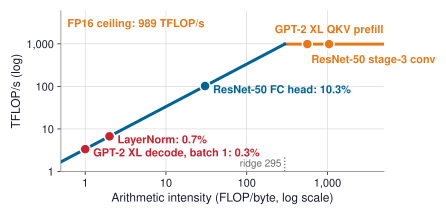
\includegraphics[width=\textwidth,height=3.4cm,keepaspectratio]{layers_step4}
    \end{column}
    \begin{column}{0.56\textwidth}
      {\small\textcolor{lightgray}{NEXT LECTURE \textbar{} BENCHMARKING}}\\[0.5cm]
      {\LARGE\bfseries Every vendor claims to be fastest. How do we measure fairly?}
    \end{column}
  \end{columns}
  \note{[0.5 min] Both parts of this lecture reasoned from ceilings and models. Lecture 12 measures where a real run sits below those ceilings, and how to compare chips when each vendor quotes a different peak.}
\end{frame}

\end{document}
